\chapter{Design}

\section{Overview of the Approach}
Our concept includes the following systems illustrated in Figure \ref{fig:frameworks}. We rely on two existing frameworks in our work, the Train Benchmark and MONDO-SAM frameworks, furthermore, we elaborate \framework, the \textit{MONDO-Metrics-Based Analysis of Performance} framework and the Homogeneous Graphs Benchmark.
%todo mondo sam cite
\begin{figure}[!ht]
	\centering
	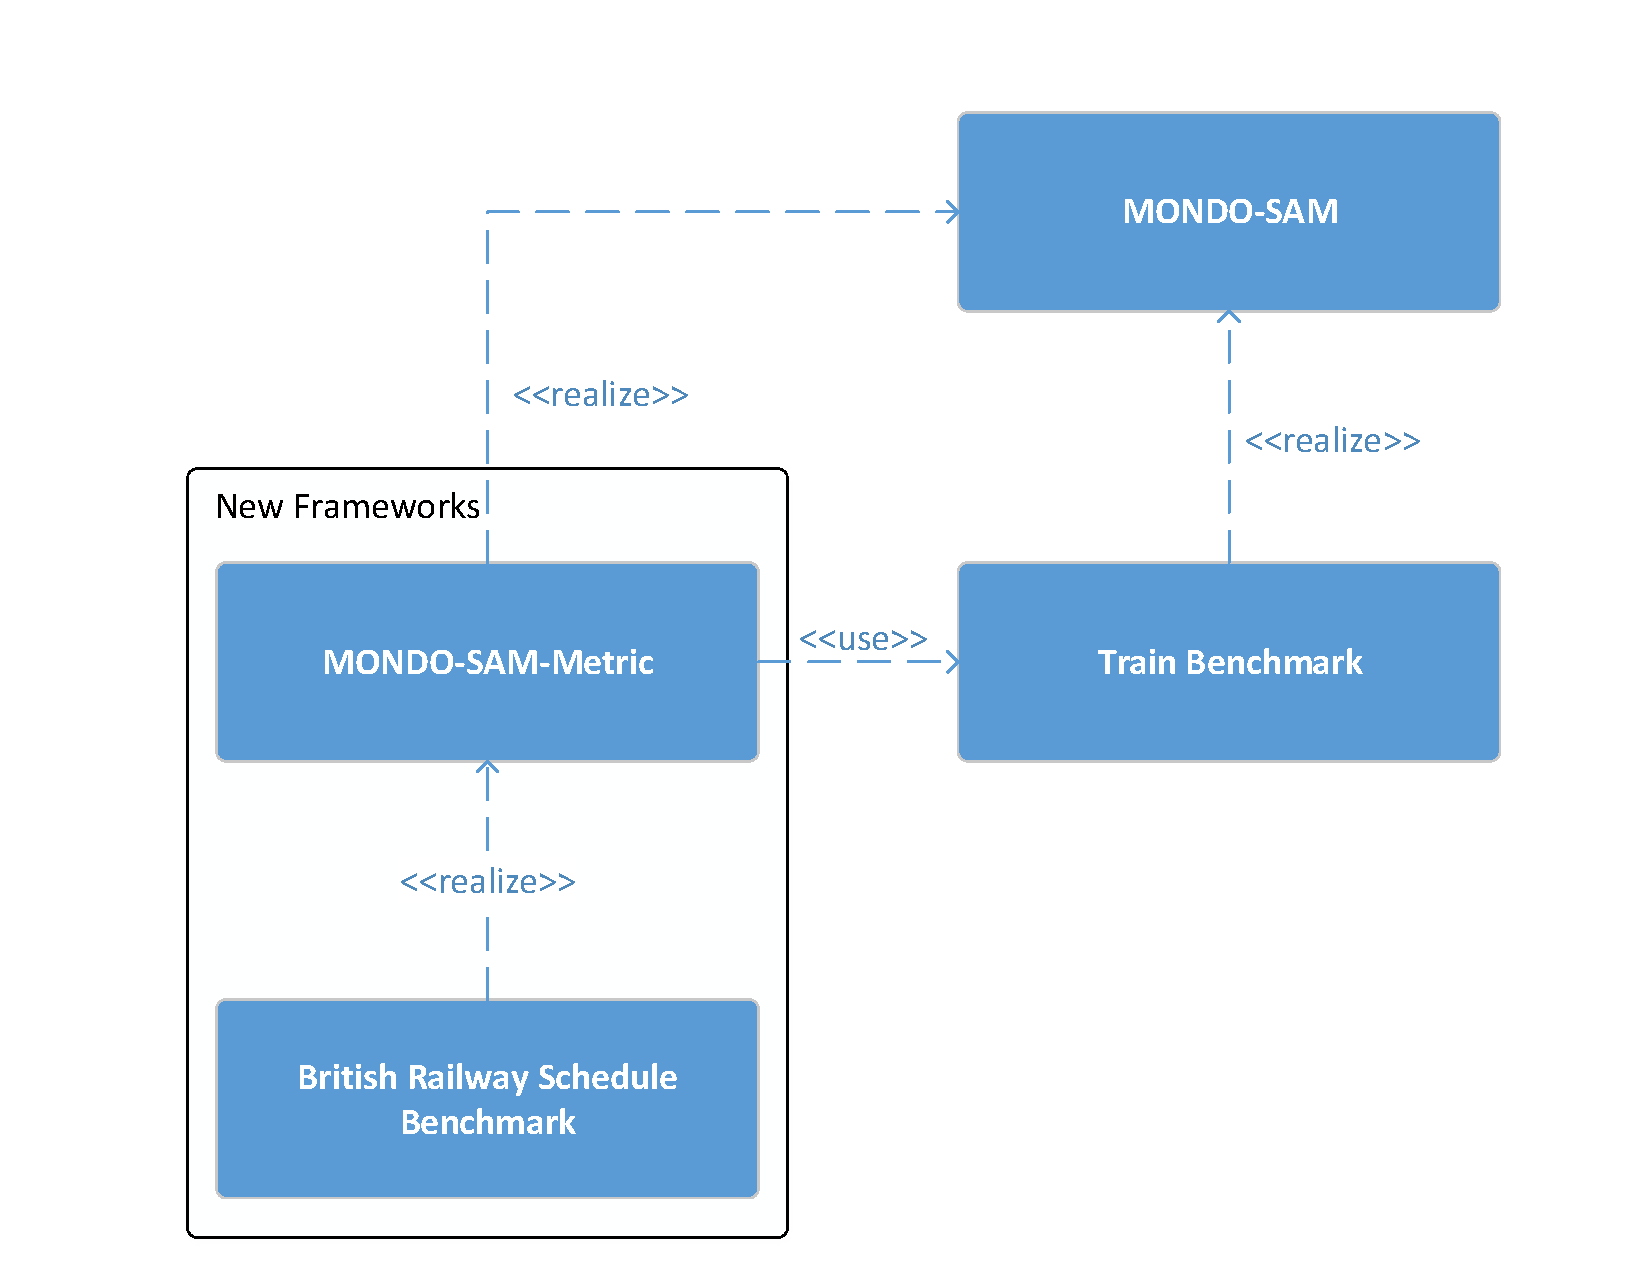
\includegraphics[width=130mm, keepaspectratio]{figures/frameworks.pdf}
	\caption{An overview of the frameworks in our approach.}
	\label{fig:frameworks}
\end{figure}

\paragraph{MONDO-SAM}
The MONDO-SAM framework was created under the project MONDO~\cite{mondo} with the motivation to provide a common benchmark framework in Model Driven Engineering (MDE) for benchmark developers~\cite{mondo-sam}. \sam can be considered as an abstract layer that proposes an evaluation engine to execute arbitrary workflows independently on the current workload, furthermore, \sam also guarantees the serialization and data visualization of the benchmark results.

\paragraph{Train Benchmark}
The Train Benchmark framework is based on the evaluation engine provided by \sam, and it proposes a benchmark for measuring continuous model validations and transformations, introduced in Section \ref{sec:train}.

\paragraph{\framework}
\framework extends \sam with further features, as it provides a framework for analyzing model and performance relationships in the light of an arbitrary workload by characterizing the performance quantitatively with model related metrics. Similarly to \sam, \map is an abstract framework and can be extended by an arbitrary benchmark case.

\paragraph{Homogeneous Graphs Benchmark}

\begin{figure}[!ht]
	\centering
	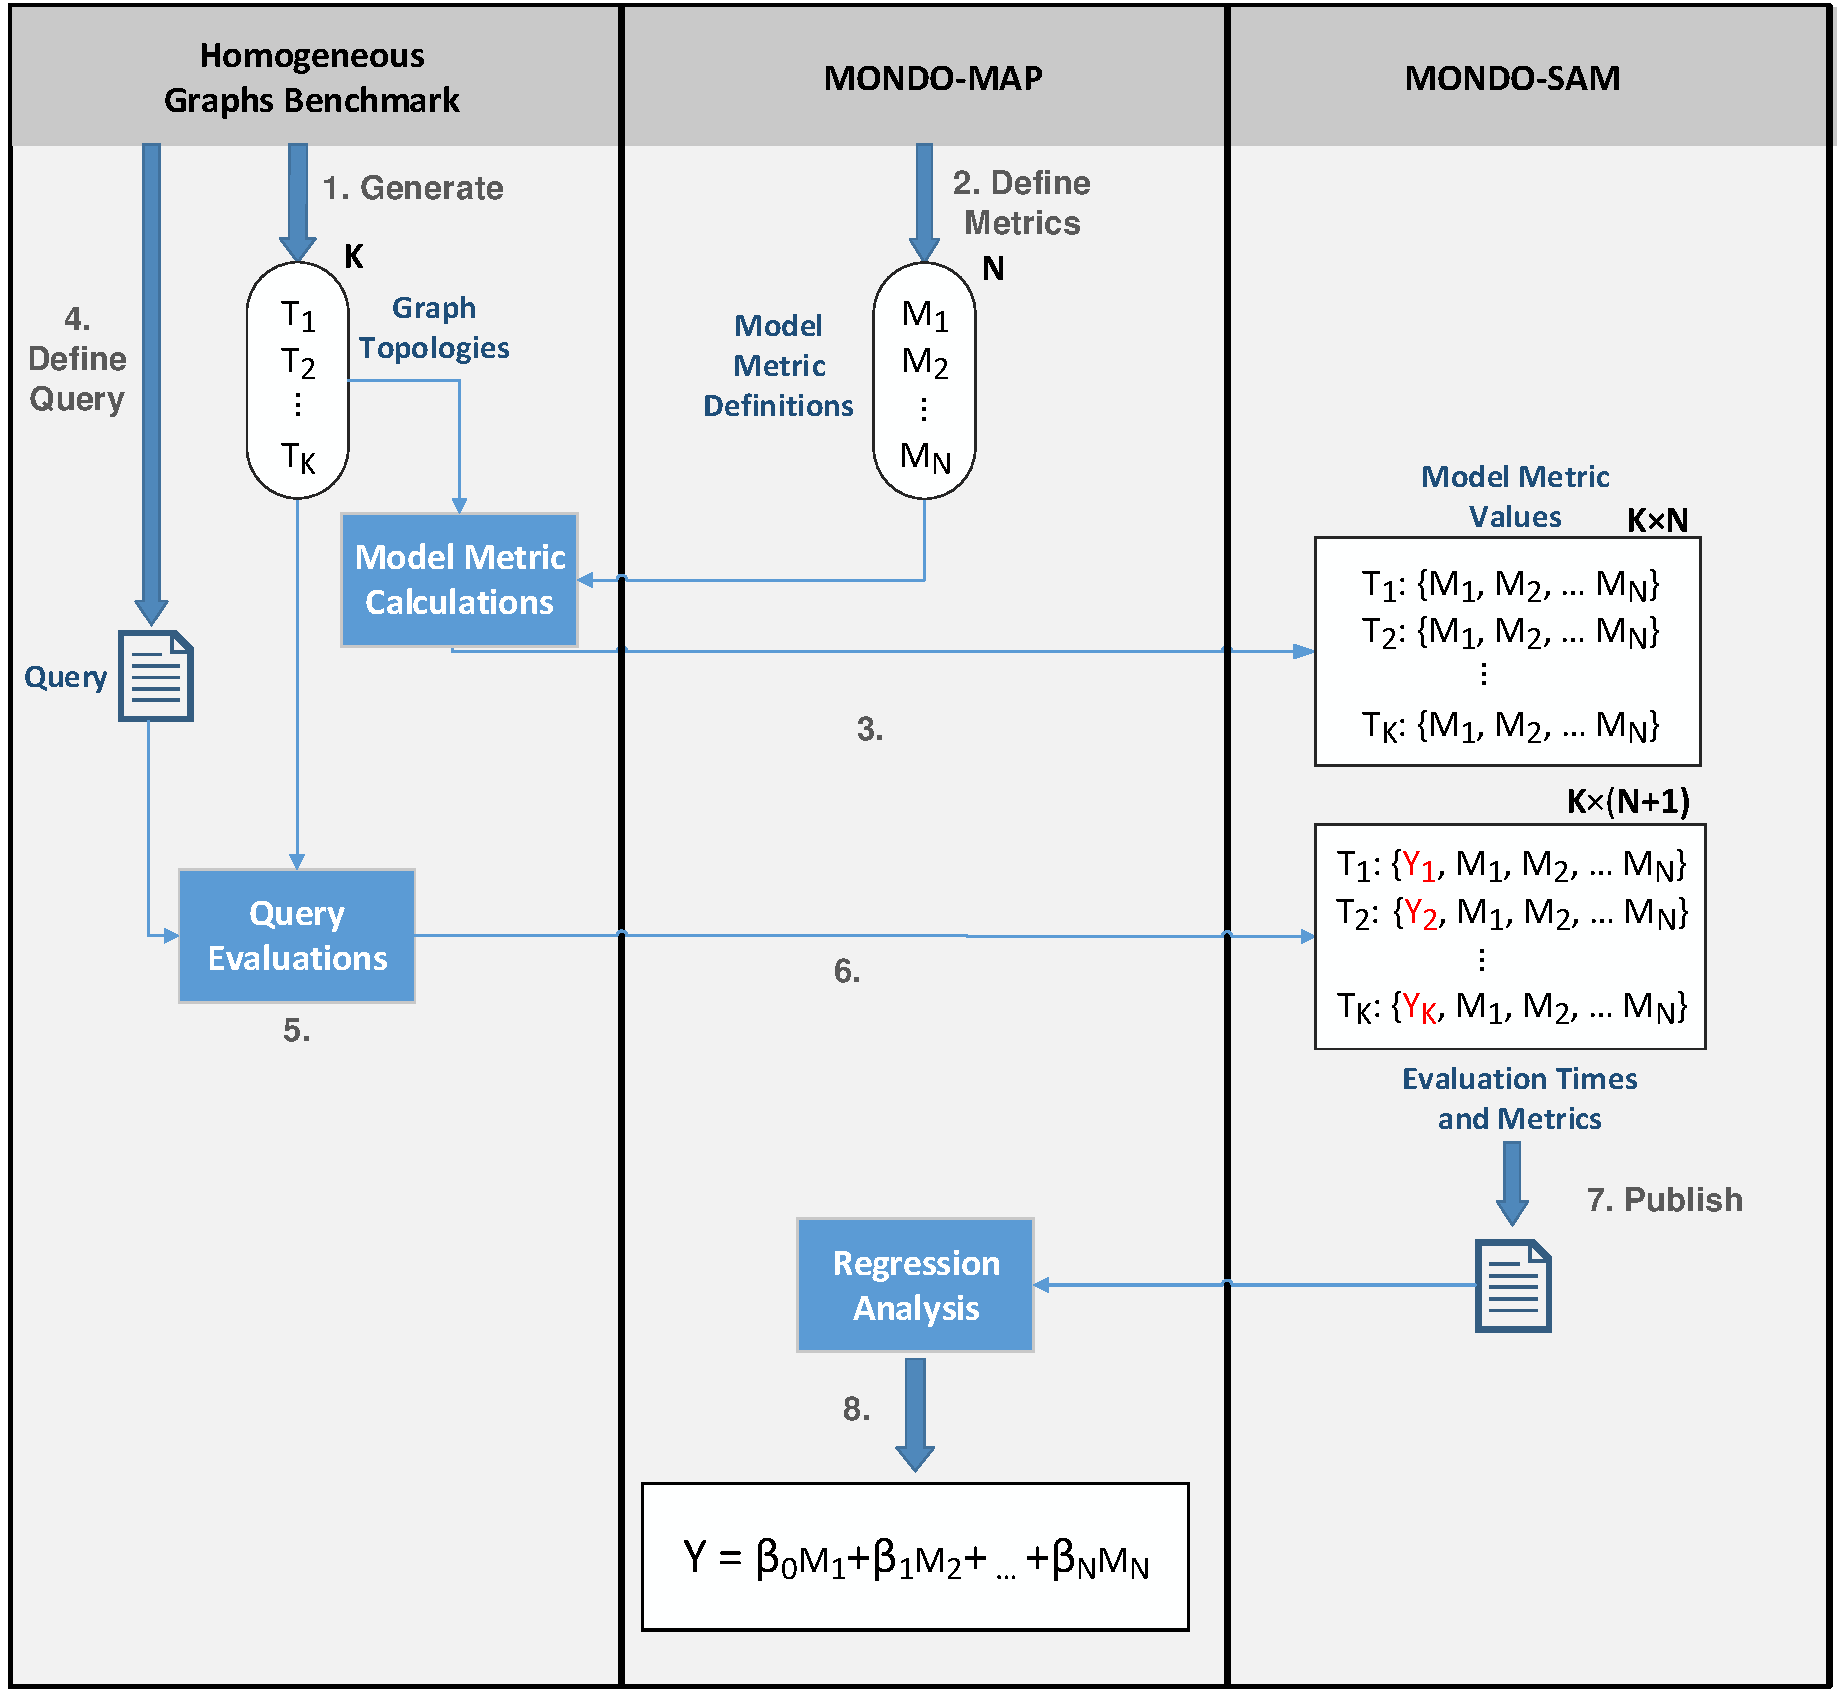
\includegraphics[width=140mm, keepaspectratio]{figures/approach.pdf}
	\caption{The main concept of the metric-based performance analysis.}
	\label{fig:approach}
\end{figure}

The Homogeneous Graphs Benchmark (HG Benchmark) extends the \map framework with a benchmark case for RDF databases. It generates homogeneous graphs ---well-known network topologies---and it investigates the relationships between the model metrics and performance of query evaluations with respect to an arbitrary query and database. The goal is to generate artificial graphs with various characteristics and obtain a fluctuation in their descriptive metrics, and thus showing a quantitative connection between the model metrics and performance. As Figure \ref{fig:frameworks} suggests, in the HG Benchmark we use a part of the components of Train Benchmark that are adequate for our purpose as well.

Figure \ref{fig:approach} illustrates the main concept of our work. First, the HG Benchmark generates different $K$ number of graph topologies. Using the graph metric definitions from \map (2.), we calculate the descriptive metrics for every topology in step 3. As it is showed, every topology contains an own values for every $N$ number of metrics, and they are stored in \sam. In the next two steps (4-5.) we define a query and evaluates it on every topology in the particular RDF database that we intend to measure. The measurement result is the query evaluation time ($Y$) that represents another variable belonging to the topologies besides their metrics (6.). As it was mentioned before, the \sam framework is responsible for publishing the benchmark results(7.). Finally, in \map we analyze the results by creating regression models to estimate the influence of metrics to the performance.

%\subsubsection{Challenges}

%Three challenges can be found in our research. At first, we have to provide a solution in the HG benchmark to generate models with different %characteristics that impact the performance of a particular query and cause a deviation in evaluation time. 
%Second, we have to find model metrics that are able to characterize the models individually. Furthermore, these attributes must be suitable to %create quantitative relationships among them and the evaluation times.

\section{Models and Metrics}
\subsection{Real-Life Networks}

%todo copy heavy tail to background
In the discipline of graph theory, the internal structures of real-life networks are comprehensively investigated. The main approach in the analysis of these networks is to explore the degree distributions and study the specific metrics---typically the clustering coefficients, average degrees, average shortest paths---that are suited to characterize the graphs appropriately. Based on the degree distributions and metrics, one can draw conclusion how a particular real-life network shows a similar characteristic to the well-known topologies such as the random graph, scale-free model, small-world model of Watts-Strogatz, or hierarchical network.\\
For example, the network of world-wide-web is studied in~\cite{www1} and~\cite{www2} as well, and the authors observe that the degree distribution of the \textit{www} follows a power-law distribution with a heavy tail\footnote{The concept of heavy tail means that there is a larger probability of receiving significantly higher values, than it is normally expected~\cite{heavy_tail}.}, which indicates the presence of web pages with significantly higher degrees than the average degree. Since the probability of occurrences of these web pages is considerably low, the connectivity of the world-wide-web can be represented by the scale-free model of Barabási and Albert.

%todo insert table from StatisticalMechanics_Rev of Modern Physics 74, 47 (2002)

More examples can be found in the study of Barabási and Albert~\cite{statistical_mechanics}, as they review the advances of different publications and investigate the characteristics of different real-life networks (Table). Empirical results prove that the \textit{movie actor collaboration network}, \textit{cellular networks}, \textit{phone call} and \textit{citation} networks also follow power-law distributions. Many of the studied networks can be considered as scale-free models, however, a part of these graphs---for example the network of movie actors---also show small-world properties and high clustering coefficient in their connectivity similarly to the Watts-Strogatz or hierarchical topology.

As far as the Watts-Strogatz model---and the random graph---are concerned, their specific degree distribution---Poisson---rarely appears in the real-life networks, as it is emphasized in~\cite{random_study}. Actually, none of the artificial topologies can be identified perfectly to real-life models, however, the ensemble of the specific attributes of these well-known topologies are frequently appear in them. As a conclusion, we conjecture that the characteristics belonging to the well-known topologies are the foundations of our solution, namely, finding those representative metrics of graphs that are suited to characterize not only the model appropriately, but the relationship between model and performance as well.

\subsection{Network Topologies and Representative Metrics}

Barabási and Albert inspect the natures of the well-known graph topologies in~\cite{statistical_mechanics}, such as the random graph, scale-free and the Watts-Strogatz model. As a main result, they observe that there are significant differences among the topologies regarding specific graph metrics. Based on their study and the research of hierarchical graphs~\cite{hierarchical}, the following metric deviations are assumed	between the four topologies, illustrated in Table \ref{tab:topology_metrics}. The random graph is considered as a reference point, and every value is compared to its metrics by assuming that the networks are in the same size.
\begin{table}[ht]
	\footnotesize
	\centering
	\begin{tabular}{ l c c c c}
		\toprule
		Metric & Random & Hierarchical & Scale-free & Watts-Strogatz \\ 
		\midrule 
		\textbf{Max Degree} & $\bullet$ & $\bullet$$\bullet$$\bullet$ & $\bullet$$\bullet$$\bullet$ & $\bullet$ \\ \hline
		\textbf{Clustering Coefficient} & $\bullet$ & $\bullet$$\bullet$$\bullet$ & $\bullet$ & $\bullet$$\bullet $\\ \hline
		\textbf{Avg Shortest Path Length} & $\bullet$ & $\bullet$$\bullet$ & $\bullet$ & $\bullet$$\bullet$ \\ \hline
		\bottomrule
	\end{tabular}
	\caption{Graph topologies and their descriptive metrics}
	\label{tab:topology_metrics}
\end{table}
%todo describe bullets in detail
As Table \ref{tab:topology_metrics} demonstrates, each topology can be characterized by different metric values, which leads to the assumption that if the diversity between the topologies may cause fluctuations in the performance of a particular query evaluation, then these metrics are adequate to characterize the model and performance relationships quantitatively.

%todo use lattice ref in background
%todo emphasize lattice, random and p value in background, maybe add a picture as well

However, the values of metrics in Table \ref{tab:topology_metrics} are misleading due to the reason that the metrics of the Watt-Strogatz model highly depend on the initialization of the network, namely, the value of $p$ probability that is used in the generation.

\begin{figure}[!ht]
	\centering
	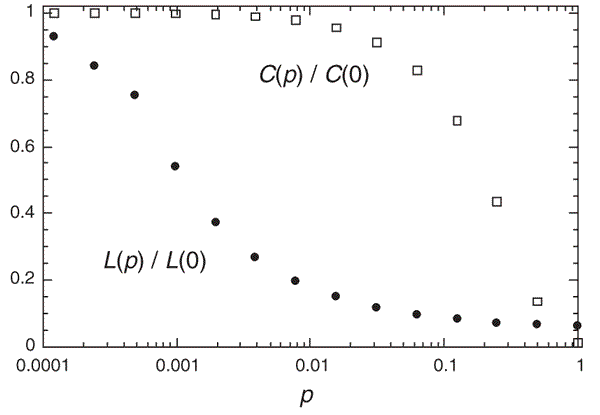
\includegraphics[width=100mm, keepaspectratio]{figures/ws_metrics.png}
	\caption{Characteristic path length $L(p)$ and clustering coefficient $C(p)$ of Watts-Strogatz model}
	\label{fig:ws}
\end{figure}

By modifying $p$, the Watts-Strogatz model represents a bridge between a lattice and a random graph. As Figure \ref{fig:ws} illustrates\footnote{The original figure can be found in~\cite{ws_metrics}.}, the clustering coefficient ($C(p)$) and average shortest path ($L(p)$) metrics are changed with respect to $p$ scaling. The values are normalized by $L(0)$ and $C(0)$ that represent the clustering coefficient and average shortest path metrics for a lattice graph. As a conclusion, the Watts-Strogatz model shows significant deviations in these two metrics in the light of the $p$ probability value. 

%todo add betweenness reference to background
Besides the models in Table \ref{tab:topology_metrics}, the metrics also require modifications. The problem is that the maximum degree metric alone does not include a comprehensive information about the internal structure of the network, since it does not emphasize the role of a node with maximum degree in the connectivity of the graph. Hence, we introduce another metric---the \textit{betweenness centrality}---which characterizes adequately the importance of a higher degree, since the higher value of betweenness centrality belongs to a vertex, the more shortest paths include that node, symbolizing that node represents the center in the graph.

After these minor modifications, the topologies and the related metrics are showed in the extended Table \ref{tab:topology_metrics2}. The \textsf{WS-x} abbreviations symbolize the Watts-Strogatz models indicating that the $p$ value is equal to $x$. The values of the betweenness centrality are determined by our initial conjecture considering that the center node in a hierarchical network and the \textit{hubs} in a scale-free model may occur more times in the shortest paths due to the fact that they have higher degrees. The main conclusion is that we can achieve a higher deviation among the metric values by using these topologies, and thus, in the following we concentrate on these networks.
\begin{table}[ht]
	\footnotesize
	\centering
	
	\begin{tabular}{ l c c c c c c}
		\toprule
		Metric & Random & Hierarchical & Scale-free & WS-0.1 & WS-0.01 & WS-0.001 \\ 
		\midrule 
		\textbf{Max Degree} & $\bullet$ & $\bullet$$\bullet$$\bullet$ & $\bullet$$\bullet$$\bullet$ & $\bullet$ & $\bullet$ & $\bullet$ \\ \hline
		\textbf{Clustering Coefficient} & $\bullet$ & $\bullet$$\bullet$$\bullet$ & $\bullet$ & $\bullet$$\bullet$ & $\bullet$$\bullet \bullet$ & $\bullet$$\bullet$$\bullet$\\ \hline
		\textbf{Avg Shortest Path Length} & $\bullet$ & $\bullet$$\bullet$ & $\bullet$ & $\bullet $ & $\bullet \bullet$ & $\bullet$$\bullet$$\bullet$\\ \hline
		\textbf{Betweenness Centrality} & $\bullet$ & $\bullet$$\bullet$$\bullet$ & $\bullet$$\bullet$ & $\bullet$ & $\bullet$ & $\bullet$\\ \hline
		\bottomrule
	\end{tabular}
	\caption{Graph topologies and their descriptive metrics with extensions}
	\label{tab:topology_metrics2}
\end{table}

\section{Metric and Performance Comparison}

Showing an appropriate performance and metric relationship is an essential part of our approach. The first notion is the search of correlations between the metrics and performance.

A similar problem is studied in~\cite{algebraic1} and~\cite{algebraic2}, where the authors generate well-known topologies and inspect the connectivity and robustness of the networks. In their case, a network is said to be robust if its performance is not sensitive to the changes in topology. In~\cite{algebraic1}, the algebraic connectivity metric is studied to search robustness and metric relationships, however, they show that the algebraic connectivity is not trivially correlated to the robustness of the network.\\
The authors in~\cite{algebraic2} investigate the impact of betweenness centrality, algebraic connectivity and average degree to robustness, and they also draw the conclusion that there is no unique graph metric to satisfy both connectivity and robustness objectives while keeping a reasonable complexity, since each metric captures some attributes of the graph.

Partly based on the advances of these two publications and our initial assumption of the topologies and their metrics (Table \ref{tab:topology_metrics2}), we expect that we cannot find a correlation between one metric and the performance, hence, we conjecture that only the ensemble of more metrics is suited to find relationship.

In order to find quantitative connections, we use regression analysis to show how the various metrics impact the performance. 

\subsection{Sample Choosing}

By using regression analysis on a sample, it is inevitable to regard the sample to be unbiased. In our case, a bias in a sample of graph topologies means a fluctuation in the size of the models. Obviously, one topology in the sample with larger amount of nodes can bias the connection between the models and the performance, therefore, our framework must support the generation of \textit{uniform} models with respect to the amount of nodes and edges, even in the case of different topologies as well.\footnote{From now on, under the concept of uniform models we mean models with approximately equal number of nodes and edges, despite the diversity of their internal structures.}
